\documentclass[twocolumn]{IEEEtran}
\usepackage{graphicx}
\usepackage[utf8x]{inputenc}
\usepackage{times}
\usepackage{amssymb,amsfonts}
\usepackage[tbtags]{amsmath}
\usepackage{cite}
\usepackage{pict2e}
\usepackage{float}
\usepackage{lscape}
\usepackage[all]{xy}
\usepackage{graphics,graphicx,color,colortbl}
\usepackage{times}
\usepackage{subfigure}
\usepackage{wrapfig}
\usepackage{multicol}
\usepackage{cite}
\usepackage{url}
\usepackage[tbtags]{amsmath}
\usepackage{amsmath,amssymb,amsfonts,amsbsy}
\usepackage{listings}
\usepackage{bm}
%\usepackage{algorithm}
%\usepackage{algorithmic}
\usepackage[centerlast, small]{caption}
\usepackage[colorlinks=true, citecolor=blue, linkcolor=black, urlcolor=black, breaklinks=true]{hyperref}
\hyphenation{ele-men-tos he-rra-mi-en-ta cons-tru-yen trans-fe-ren-ci-a pro-pu-es-tas si-mu-lar vi-sua-li-za-cion}

\begin{document}
\title{Comparación de aplicaciones en Hardware y Software}
\author{José Alejandro Logreira Ávila Código: $261722$\\
	David Ricardo Martínez Hernández Código: $261931$\\
	Edwin Fernando Pineda Vargas Código: $262100$}
\maketitle
\markboth{Universidad Nacional de Colombia}{}
\floatname{algorithm}{Algoritmo}
\begin{keywords}
 ALU, Ciclos de reloj, Hardware, Operandos, Multiplicación, Software, Sumas Sucesivas.
\end{keywords}
\begin{abstract}
 En esta práctica se busca encontrar las diferencias en implementación de una solución tanto en hardware como en software.
\end{abstract}

\section{Introducción}
\noindent
Existen varias formas de implementar algoritmos en MIPS. Durante esta práctica, se implementará el algoritmo mediante sumas sucesivas y mediante la instrucción mul o muli. Para verificar esto, se harán simulaciones mediante el GTK wave, con ello buscamos el tiempo de respuesta de cada casoy así podremos realizar la correspondiente comparación.

\section{Tareas desarrolladas por software en el LM32}\label{sumas}
\noindent
El código siguiente realiza la tarea de multiplicación, usando el algoritmo de sumas sucesivas. Este tipo de implementación de la multiplicación supone que no existe un módulo aritmético dedicado a la  multiplicación en el procesador, y por tanto la forma de desarrollar una operación de multiplicación es mediante el uso recursivo de los recursos que sí tiene, como la unidad aritmética lógica.
\lstset{numbers=left, numberstyle=\tiny, stepnumber=1, numbersep=1pt}
\begin{lstlisting}[firstnumber=7, caption=Codigo inicial, label=code1]
#include "soc-hw.h"
int main(void){
   volatile uint32_t a,b,c,i;
   a = 10;
   b = 13;
   c = 0;
   while (i<b) {
      c = c + a;
      i = i + 1;
               }
   return 0;
}
\end{lstlisting}
\noindent
Este algoritmo representa la forma de realizar tareas por software ya que ejecuta instrucciones sencillas, que hacen uso de los recursos simples disponibles en el procesador (suponiendo que no dispone del módulo multiplicador), para realizar tareas más complejas y elaboradas.\\
En la multiplicación de los enteros $10$ y $13$, se está sumando sucesivamente $10$, $13$ veces, por lo que estas sumas son las que debemos evidenciar como resultados en la salida de la ALU. Se declaran las variables de tipo volátil para poderlas observar en el simulador GTKwave.\\
La siguiente imagen muestra el comienzo de la operación, donde se inicializa uno de los registros con el sumando $10$:
\begin{figure}[H]
	\centering
		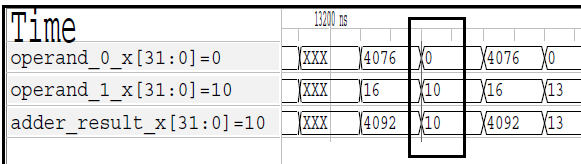
\includegraphics[scale=0.5]{01.png}
	\caption{Simulación obtenida en \textbf{GTKwave} de la multiplicación por sumas sucesivas.}
	\label{fig1}
\end{figure}
\noindent
Las siguientes imágenes muestran la primera iteración de la suma, y algunas de las iteraciones posteriores. Finalmente se obtiene el resultado en la iteración final, mostrada en la última imagen Fig. \ref{fig15}.\\
\begin{figure}[]
    \begin{minipage}[t]{1cm}
    \centering
        \subfigure[]{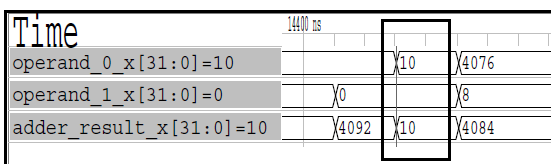
\includegraphics[scale=0.6]{02.png}}
    \end{minipage}\\
    \begin{minipage}[H]{1cm}
    \centering
        \subfigure[]{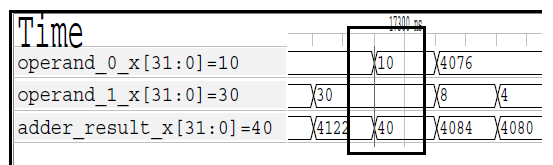
\includegraphics[scale=0.62]{03.png}}
    \end{minipage}\\
    \begin{minipage}[H]{1cm}
    \centering
        \subfigure[]{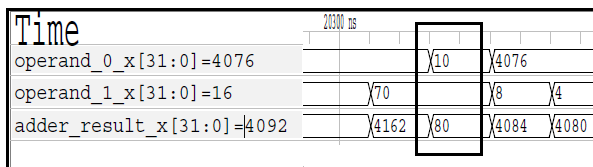
\includegraphics[scale=0.57]{04.png}}
    \end{minipage}\\
    \begin{minipage}[H]{1cm}
    \centering
        \subfigure[]{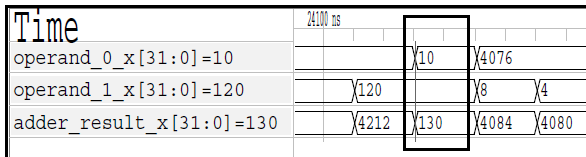
\includegraphics[scale=0.58]{05.png}}
    \end{minipage}
\caption{Simulación obtenida en \textbf{GTKwave} de la multiplicación por sumas sucesivas.}
\label{fig15}
\end{figure}
\noindent
La TABLA \ref{tab1} a continuación muestra los tiempos de ejecución del programa según se observó en el simulador GTKwave.
\begin{table}[H]
	\centering
\begin{tabular}{|c|c|c|c|}\hline
\textbf{Operación} & \textbf{Tiempo} & \textbf{Tiempo de la OP} & \textbf{Tiempo} \\
 & \textbf{de la OP} & \textbf{Anterior} & \textbf{Acumulado} \\ \hline
Carga $10$ en registro & $13230$ & $0$ & $0$ \\ \hline
$0+10$ & $14430$ & $1200$ & $1200$ \\ \hline
$10+10$ & $15770$ & $1340$ & $2540$ \\ \hline
$10+20$ & $16560$ & $760$ & $3300$ \\ \hline
$10+30$ & $17290$ & $760$ & $4060$ \\ \hline
$10+40$ & $18050$ & $760$ & $4820$ \\ \hline
$10+50$ & $18810$ & $760$ & $5580$ \\ \hline
$10+60$ & $19570$ & $760$ & $6340$ \\ \hline
$10+70$ & $20330$ & $760$ & $7100$ \\ \hline
$10+80$ & $21090$ & $760$ & $7860$ \\ \hline
$10+90$ & $21850$ & $760$ & $8620$ \\ \hline
$10+100$ & $22610$ & $760$ & $9380$ \\ \hline
$10+110$ & $23370$ & $760$ & $10140$ \\ \hline
$10+120$ & $24130$ & $760$ & $10900$ \\ \hline
    \end{tabular}
	\caption{Tiempo de la multiplicación por sumas sucesivas para el procesador $LM32$.}
	\label{tab1}
\end{table}
\noindent
Como es evidente en la tabla, existe una periodicidad en el tiempo que demora cada iteración de suma. El tiempo total de ejecución de la suma sucesiva es de $10900$ nanosegundo, $10,9$ microsegundos. Este tiempo crecerá linealmente conforme crece la magnitud de los operandos.

\section{Tareas implementadas en hardware en el LM32}
\noindent
Se utilizó el siguiente código en C para implementar la multiplicación 
\lstset{numbers=left, numberstyle=\tiny, stepnumber=1, numbersep=1pt}
\begin{lstlisting}[firstnumber=7, caption=Codigo inicial, label=code1]
#include "soc-hw.h"
int main(int argc, char **argv){
   volatile unsigned int multiplicador =10;
   volatile unsigned int multiplicando =13;
   volatile unsigned int producto = 0;
   producto = multiplicador*multiplicando;
   return 0;
}
\end{lstlisting}
\noindent
El resultado de la simulación se observa en la figura \ref{fig2}, en dicha figura los datos ingresan a los registros en $14150$ nanosegundos ($14.150 \mu s$) y el resultado se obtiene a los $14170$ nanosegundos ($14.170 \mu s$), esto quiere decir que solo se demora un ciclo para dar la respuesta.
\begin{figure}[H]
	\centering
		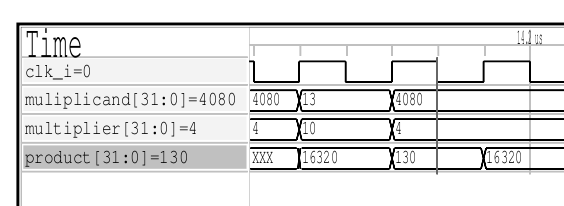
\includegraphics[scale=0.45]	{simulation_multiplication.png}
	\caption{Simulación obtenida en \textbf{GTKwave} de la multiplicación directa.}
	\label{fig2}
\end{figure}
\noindent
Comparado con el proceso de la sección pasada (ver ~\ref{sumas}) el tiempo de ejecución es menor porque en el \textit{main.s} llama a la función \textit{\_\_ mulsi3} por medio de la instrucción \textit{calli}, esto hace que se reduzca el tiempo de ejecución de $13$ ciclos a un solo ciclo (para este caso en particular).

\section{Conclusiones}
\begin{itemize}
\item No cabe duda que el rendimiento en tiempo de realizar tareas por hardware es mucho más eficiente que por software.
\item El lograr eficiencia implementando hardware, también significa un aumento de recursos en el mismo. Lo cual en el ámbito comercial se traduce en costos más elevados.
\item Esta idea de desempeño versus recursos de hardware, es también evidente en la llamada Arquitectura del Set de instrucciones, en donde cada instrucción realizará una tarea sencilla o compleja conforme se dispongan de recursos de Hardware.
\end{itemize}


\bibliographystyle{ieeetran}
\begin{thebibliography}{99}
\bibitem{patterson} Patterson, David \& Hennessy John
{\em "`Computer Organization And Design - The Hardware-Software Interface"'}.
Kindle Edition, Fourth Edition, 2006.

\bibitem{page1} \url{http://www.latticesemi.com/products/intellectualproperty/ipcores/mico32/index.cfm}

\bibitem{page2} \url{http://www.linuxencaja.net/wiki/Arquitectura_LM32_JPRR_%28261744%29}
\end{thebibliography}
\end{document}